% !TeX document-id = {0be8c18c-9430-4e9a-bdd9-12beadebfebc}
% !TeX TXS-program:bibliography = txs:///biber
\documentclass[11pt]{beamer}

\usepackage[brazilian]{babel}

\uselanguage{portuguese}
\languagepath{portuguese}
\deftranslation[to=portuguese]{Theorem}{Teorema}
\deftranslation[to=portuguese]{theorem}{teorema}
\deftranslation[to=portuguese]{Example}{Exemplo}
\deftranslation[to=portuguese]{example}{exemplo}
\deftranslation[to=portuguese]{Lemma}{Lema}
\deftranslation[to=portuguese]{lemma}{Lema}
\deftranslation[to=portuguese]{Corollary}{Corolário}
\deftranslation[to=portuguese]{corollary}{corolário}
%\deftranslation[to=portuguese]{and}{e}
\newtheorem{proposition}{Proposição}
\newtheorem{assumption}{Hipótese}

\usepackage[utf8]{inputenc}
\usepackage[T1]{fontenc}
\usepackage{lmodern}
\usepackage{amsmath}
\usepackage{amssymb}
\usepackage{mathtools}
\usepackage{color}
\usepackage{pgfplots}
\usepackage{tikz}
\usepackage{subcaption}
%\usepackage{appendixnumberbeamer}

\newenvironment{transitionframe}{
	\setbeamercolor{background canvas}{bg=yellow}
	\begin{frame}}{
	\end{frame}
}
\usetheme{default}
\usefonttheme{structuresmallcapsserif}

%% I use a beige off white for my background
\definecolor{MyBackground}{RGB}{255,253,218}
\useinnertheme[shadow]{rounded}
\setbeamercolor{block title}{bg=MyBackground}
\setbeamercolor{block body}{bg=MyBackground}
\setbeamercolor{example title}{bg=MyBackground}
\setbeamercolor{example body}{bg=MyBackground}


\newcommand{\blue}[1]{\textcolor{blue}{#1}}
\newcommand{\red}[1]{\textcolor{red}{#1}}
\newcommand{\purple}[1]{\textcolor{purple}{#1}}
\newcommand{\gray}[1]{\textcolor{gray}{#1}}
\setbeamertemplate{navigation symbols}{}
%\setbeamertemplate{page number in head/foot}[appendixframenumber]

%\usepackage{graphics}
\usepackage{graphicx}

\definecolor{blue_emph}{RGB}{0,114,178}
\definecolor{red}{RGB}{213,94,0}
\definecolor{yellow}{RGB}{240,228,66}
\definecolor{green}{RGB}{0,158,115}
\definecolor{purple}{RGB}{204,121,167}
\definecolor{orange}{RGB}{230,159,0}
\definecolor{lightblue}{RGB}{86,180,233}

%\setbeamercolor{frametitle}{fg=blue}
%\setbeamercolor{title}{fg=blue}
\setbeamertemplate{footline}[frame number]
\setbeamertemplate{navigation symbols}{} 
\setbeamertemplate{itemize items}{-}
%\setbeamercolor{itemize item}{fg=blue}
%\setbeamercolor{itemize subitem}{fg=blue}
\setbeamertemplate{enumerate items}[default]
%\setbeamercolor{enumerate subitem}{fg=blue}
\setbeamercolor{button}{bg=MyBackground,fg=blue}
\usefonttheme{structuresmallcapsserif}

%\setbeamercolor{section in toc}{fg=blue}
%\setbeamercolor{subsection in toc}{fg=red}
\setbeamersize{text margin left=1em,text margin right=1em} 


\usepackage{appendixnumberbeamer}
\usepackage{pdfpages}
\usepackage[
backend=biber,
uniquename=false,
uniquelist=false,
style=authoryear,
natbib=true
]{biblatex}
\addbibresource{../bibliography.bib}

\newenvironment{wideitemize}{\itemize\addtolength{\itemsep}{10pt}}{\enditemize}
\newenvironment{wideenumerate}{\enumerate\addtolength{\itemsep}{10pt}}{\endenumerate}
\newenvironment{halfwideitemize}{\itemize\addtolength{\itemsep}{0.5em}}{\enditemize}
\newenvironment{halfwideenumerate}{\enumerate\addtolength{\itemsep}{0.5em}}{\endenumerate}


\author{Luis A. F. Alvarez}
\title{Econometria I}
\subtitle{O estimador de Mínimos Quadrados Ordinários}
%\logo{}
%\institute{}
\date{\today}
%\subject{}
%\setbeamercovered{transparent}

\def\signed #1{{\leavevmode\unskip\nobreak\hfil\penalty50\hskip2em
		\hbox{}\nobreak\hfil(#1)%
		\parfillskip=0pt \finalhyphendemerits=0 \endgraf}}

\newsavebox\mybox
\newenvironment{aquote}[1]
{\savebox\mybox{#1}\begin{quote}}
	{\signed{\usebox\mybox}\end{quote}}

\begin{document}

\begin{frame}[plain]
	\maketitle
\end{frame}
\begin{frame}{Ambiente}
	\begin{itemize}
		\item Pesquisador observa $n$ pares $(Y_i,X_i)$, $i=1\ldots, n$, para os quais supõe um modelo linear da forma:
		\begin{equation}
			\label{eq_line}
			Y_i = X_i'\beta + \epsilon_i\, \ldots  i=1,\ldots n\, ,
		\end{equation}
		onde $\beta\in \mathbb{R}^k$ é um parâmetro desconhecido, e $\epsilon_i$, $i=1,\ldots, n$ são variáveis aleatórias não observadas.
		\begin{itemize}
			\item Recorde-se, da última aula, que cabe ao pesquisador postular o modelo e a interpretação dos coeficientes.
			\item No caso mais comum, $(Y_i,X_i) \overset{d}{=} (Y,X)$ para $i=1,\ldots, n$, onde a distribuição de $(Y,X)$ representa a distribuição das variáveis numa população de interesse.
			\begin{itemize}
				\item Por exemplo, podemos ter que $\{(Y_i, X_i)\}_{i=1}^n$ é uma amostra aleatória de uma população com distribuição $\mathbb{P}_{Y,X}$, para a qual postulamos um modelo linear.
				\item Mas também podemos ter que as observações entre pares apresentem dependência entre si, embora com leis $\mathbb{P}_{(Y_i, X_i)}$ comuns a todo $i$.
			\end{itemize} 
			\item De modo mais geral, no entanto, pode ser que os $(Y_i,X_i)$ não possuam a mesma distribuição conjunta, mas haja uma relação comum e estável ao longo de $i$.
		\end{itemize}
	\end{itemize}
\end{frame}
\begin{frame}{Notação matricial}
	\begin{itemize}

	\item No que segue, definimos as seguintes matrizes aleatórias:
	
	$$\boldsymbol{y} = \begin{bmatrix}
		Y_1 \\
		Y_2 \\
		\vdots \\
		Y_n
	\end{bmatrix}\, , \quad \boldsymbol{X} = \begin{bmatrix}
	X_1' \\
	X_2' \\
	\vdots \\
	X_n'
	\end{bmatrix}\,, \quad \boldsymbol{\epsilon} = \begin{bmatrix}
	\epsilon_1 \\
	\epsilon_2 \\
	\vdots \\
	\epsilon_n
	\end{bmatrix}$$
	\item Com base na notação acima introduzida, podemos reescrever \eqref{eq_line} em notação matricial como:
	
	\begin{equation}
			\boldsymbol{y} = \boldsymbol{X}\beta + \boldsymbol{\epsilon}
	\end{equation}

\end{itemize}
\end{frame}

\begin{frame}{Estimador de mínimos quadrados ordinários}
\begin{itemize}
	\item O estimador de mínimos quadrados ordinários de $\beta$, denotado por $\hat{b}$, consiste em estimar $\beta$ minimizando a distância, na norma Euclidiana, entre $\boldsymbol{y}$ e uma combinação linear das colunas de $\boldsymbol{X}$, i.e. 
	
	$$\hat{b} \in \operatorname{argmin}_{b\in \mathbb{R}^k} \lVert \boldsymbol{y} - \boldsymbol{X}b \rVert_2^2 = \operatorname{argmin}_{b\in \mathbb{R}^k}\frac{1}{n}\sum_{i=1}^n (Y_i - X_i'b)^2\, ,$$
	\begin{itemize}
		\item Em outras palavras, encontramos o coeficiente $b$ que maximiza a contribuição dos $X_i$ à explicação de $Y_i$, tal qual medida pela média da distância ao quadrado entre os $Y_i$ e $X_i'b$.
	\end{itemize}
	\item Estimador é obtido como solução a uma otimização de uma função convexa, sem restrições $\implies$ condição de primeira ordem caracteriza o conjunto de soluções.
	\item Condições de primeira ordem podem ser escritas como:
	
	$$\boldsymbol{0}_{k \times 1}= \sum_{i=1}^n X_i(Y_i - X_i'b) = \boldsymbol{X}'(\boldsymbol{y}-\boldsymbol{X}b)$$
	
	
	
\end{itemize}
\end{frame}
\begin{frame}{Condição de posto e unicidade do mínimo}
Sob a condição
\begin{assumption}
	A matriz $\boldsymbol{X}$ apresenta posto $k$.
	\end{assumption}
	Temos que $\boldsymbol{X}'\boldsymbol{X}$ é invertível (por quê), de modo que  existe uma única solução ao problema de otimização, dada por:
	$$\hat{b} = (\boldsymbol{X}'\boldsymbol{X})(\boldsymbol{X}'\boldsymbol{y})\, .$$
	\begin{itemize}
		\item Condição de posto requer que nenhuma das colunas seja escrita como combinação linear das demais.
		\begin{itemize}
			\item Se a primeira entrada dos $X_i$ corresponde a um intercepto (i.e. $X_{i,1}=1$ para todo $i=1,\ldots, n$), nenhuma das colunas pode ser escrita como função afim das demais 
		\end{itemize}
		\item Observe que, como $\operatorname{rank}(\boldsymbol{X}) \leq \min\{n,k\}$, condição implica que $n \geq k$.
	\end{itemize}
\end{frame}
\begin{frame}{Um caso simples}
	\begin{itemize}
		\item Considere, para fixar as ideias, o caso em que $X_i = \begin{bmatrix}
			1 & T_i		
		\end{bmatrix}'$. 
		\item Nesse caso, a matriz $\boldsymbol{X}'\boldsymbol{X}$ é dada por:
		
		\begin{equation}
			\begin{bmatrix}
				n & \sum_{i=1}^n T_i \\
				\sum_{i=1}^n T_i & \sum_{i=1}^n T_i^2
			\end{bmatrix}
		\end{equation}
		de modo que a condição de posto é equivalente a $\widehat{{V}(T)}= \frac{1}{n}\sum_{i=1}^n T_i^2 - \left(\frac{1}{n}\sum_{i=1}^n T_i\right)^2 > 0$.
		\item Se condição de posto é satisfeita, estimador de MQO é dado por:
		
		$$\hat{b}_2 = \frac{\sum_{i=1}^n (Y_i-\bar{Y})(T_i-\bar{T})}{\sum_{i=1}^n (T_i -\bar{T})^2} = \frac{\widehat{\operatorname{cov}(T,Y)}}{\widehat{{V}(T)}}$$
	\end{itemize}
\end{frame}

	\begin{transitionframe}
	\centering
	\Huge{MQO: Propriedades Algébricas}
\end{transitionframe}

\begin{frame}{Matriz de projeção}
\begin{itemize}
	\item Definimos a matriz de projeção de $\boldsymbol{X}$ como:
	
	$$P = \boldsymbol{X}(\boldsymbol{X}'\boldsymbol{X})^{-1}\boldsymbol{X}'$$
	\begin{itemize}
		\item Observe que a matriz de projeção é tal que $X\hat{b} = P\boldsymbol{y}$.
		\item $P\boldsymbol{z}$ é a projeção (em termos de minimização da distância Euclidiana) de $\boldsymbol{z} \in \mathbb{R}^n$ no espaço gerado pelas colunas de $\boldsymbol{X}$.
	\end{itemize}
	\item Matriz de projeção tem as seguintes propriedades:
	\begin{itemize}
		\item Simétrica.
		\item Idempotente ($P^2=P$).
		\item Os autovalores de $P$ são ou $0$ ou $1$.
		\item $\operatorname{trace}(P) = k = \operatorname{rank}(P)$.
	\end{itemize}
\end{itemize}
\end{frame}
\begin{frame}{Matriz residualizadora}
	\begin{itemize}
		\item A matriz residualizadora (\textit{residual-maker}) de $X$ é dada por:
		$$M = (I-P)$$

		\item Matriz residualizadora tem as seguintes propriedades:
		\begin{itemize}
		\item Simétrica.
		\item Idempotente ($M^2=M$).
		\item Os autovalores de $M$ são ou $0$ ou $1$.
		\item $\operatorname{trace}(M) = n-k = \operatorname{rank}(M)$.
		\item $\boldsymbol{X}'M  = 0 $, $M\boldsymbol{X}=0$, $PM=MP=0$.
	\end{itemize}
	\item Matriz residualizadora devolve o erro de projeção $\boldsymbol{z} - {P}\boldsymbol{z}$.
	\begin{itemize}
		\item Como ${P}\boldsymbol{z}$ é o minimizador da distância Euclidiana no espaço gerado pelas colunas de $\boldsymbol{X}$,temos que: $$(\boldsymbol{M}\boldsymbol{z})\cdot(\boldsymbol{X}\boldsymbol{l}) = \boldsymbol{z}'M\boldsymbol{X}\boldsymbol{l} = 0\,\quad \forall \boldsymbol{z}\in \mathbb{R}^n, \boldsymbol{l} \in \mathbb{R}^k \, .$$
	\end{itemize}
\end{itemize}
\end{frame}

\begin{frame}{Visualização gráfica}
	\centering
	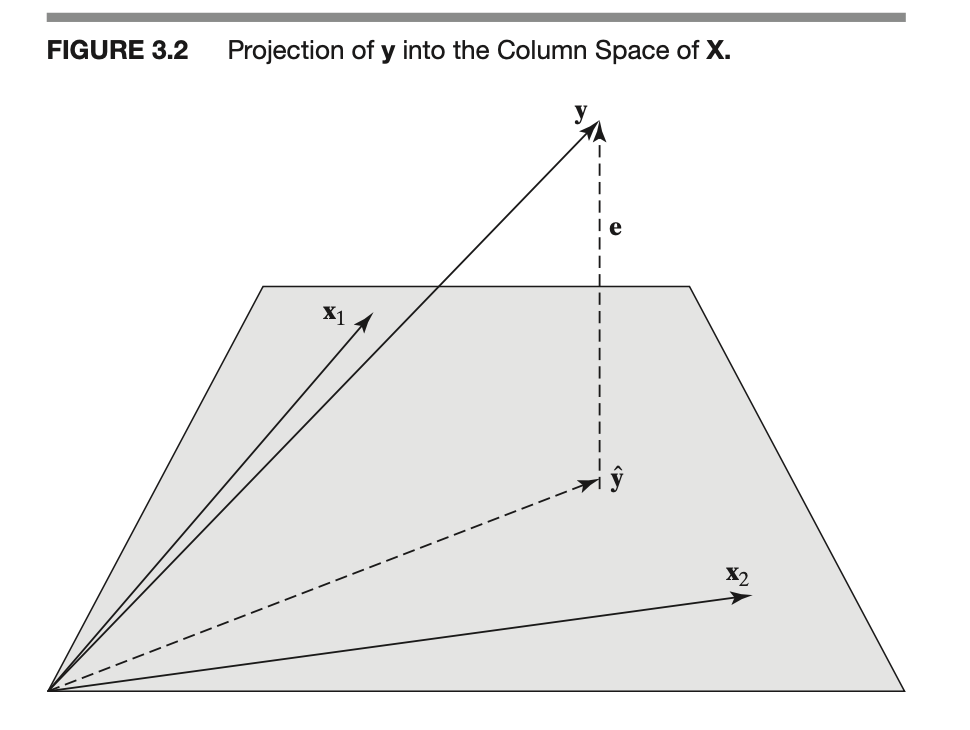
\includegraphics[scale=0.5]{plots/projecao.png}
\end{frame}

\begin{frame}{Fórmula da inversa particionada}
	\begin{itemize}
		\item 		Suponha que particionemos a matriz $\boldsymbol{X} = \begin{bmatrix}
			\boldsymbol{X}_1 & \boldsymbol{X}_2
		\end{bmatrix}$ onde $\boldsymbol{X}_1$ e $\boldsymbol{X}_2$ são matrizes de dimensão $n \times k_1$ e $n \times k_2$.
		\item Nesse caso, a fórmula da inversa particionada nos indica que:
		
	
	\begin{equation*}
			\footnotesize
		\begin{aligned}
			 (\boldsymbol{X}'\boldsymbol{X})^{-1} = \begin{bmatrix}
				\boldsymbol{X_1}'\boldsymbol{X}_1 & 	\boldsymbol{X_1}'\boldsymbol{X}_2 \\
				\boldsymbol{X_2}'\boldsymbol{X}_1 & 	\boldsymbol{X_2}'\boldsymbol{X}_2
			\end{bmatrix}^{-1} =\\  \begin{bmatrix}
				(\boldsymbol{X}_1'\boldsymbol{X}_1)^{-1}  + 	(\boldsymbol{X}_1'\boldsymbol{X}_1)^{-1} \boldsymbol{X}_1'\boldsymbol{X}_2\boldsymbol{F}\boldsymbol{X}_2'\boldsymbol{X}_1 (\boldsymbol{X}_1'\boldsymbol{X}_1)^{-1} & -  (\boldsymbol{X}_1'\boldsymbol{X}_1)^{-1} \boldsymbol{X}_1'\boldsymbol{X}_2\boldsymbol{F}\\
				- \boldsymbol{F}\boldsymbol{X}_2'\boldsymbol{X}_1(\boldsymbol{X}_1'\boldsymbol{X}_1)^{-1} & \boldsymbol{F}\end{bmatrix}
		\end{aligned}
	\end{equation*}
	onde $\boldsymbol{F}=(\boldsymbol{X}_2'\boldsymbol{X}_2 - \boldsymbol{X}_2'\boldsymbol{X}_1(\boldsymbol{X}_1'\boldsymbol{X}_1)^{-1} \boldsymbol{X}_1'\boldsymbol{X}_2 )^{-1} = (\boldsymbol{X}_2'\boldsymbol{M}_1 \boldsymbol{X}_2)^{-1}$ onde $\boldsymbol{M}_1$ é a residualizadora de $\boldsymbol{X}_1$.
\begin{itemize}
	\item Inversa de $\boldsymbol{X}_2'\boldsymbol{M}_1 \boldsymbol{X}_2$  existe pois matriz $\boldsymbol{X}$ tem posto cheio.
\end{itemize}
\end{itemize}

\end{frame}

\begin{frame}{Teorema de Frisch-Waugh-Lovell}
\begin{itemize}
	\item 	\item Da propriedade acima, segue o importante resultado abaixo:
\end{itemize}
	\begin{theorem}[Frisch-Waugh-Lovell]
	$$\hat{b}_2 = \left(\boldsymbol{X}_2'M_1\boldsymbol{X}_2\right)^{-1}\left(\boldsymbol{X}_2'M_1\boldsymbol{y}\right) = \left((M_1\boldsymbol{X}_2)'(M_1\boldsymbol{X}_2)\right)^{-1}\left((M_1\boldsymbol{X}_2)'(M_1\boldsymbol{y})\right) $$ 
	\end{theorem}
\begin{itemize}
	\item Resultado acima nos mostra que estimadores de MQO associados a $\boldsymbol{X}_2$ em uma regressão que inclui $\boldsymbol{X}_1$ e $\boldsymbol{X}_2$ são idênticos a:
	\begin{itemize}
		\item Regredir $\boldsymbol{y}$ em $\boldsymbol{X}_1$, e guardar os resíduos $\boldsymbol{e}_y$.
		\item Para cada $j=1,\ldots k_2$, regredir a $j$-ésima coluna de $\boldsymbol{X}_2$ em $\boldsymbol{X}_1$, e guardar os resíduos ${\boldsymbol{e}_j}$.
		\item Regredir $\boldsymbol{e}_y$ em $\boldsymbol{e}_1,\ldots \boldsymbol{e}_{k_2}$ e recuperar os coeficientes.
	\end{itemize}
\end{itemize}
\end{frame}

	\begin{transitionframe}
	\centering
	\Huge{MQO: Propriedades Estatísticas em Amostras Finitas}
	

\end{transitionframe}

	\begin{transitionframe}
	\centering
		\Huge{MQO: Propriedades Assintóticas}
	
	
\end{transitionframe}

\end{document}

